\chapter{Diseño e implementación} % Main chapter title

\label{Chapter3} % Change X to a consecutive number; for referencing this chapter elsewhere, use \ref{ChapterX}

En este capítulo se detallan los criterios de diseño que se tomaron para el desarrollo del sistema y los pasos seguidos para su implementación.

\definecolor{mygreen}{rgb}{0,0.6,0}
\definecolor{mygray}{rgb}{0.5,0.5,0.5}
\definecolor{mymauve}{rgb}{0.58,0,0.82}

%%%%%%%%%%%%%%%%%%%%%%%%%%%%%%%%%%%%%%%%%%%%%%%%%%%%%%%%%%%%%%%%%%%%%%%%%%%%%
% parámetros para configurar el formato del código en los entornos lstlisting
%%%%%%%%%%%%%%%%%%%%%%%%%%%%%%%%%%%%%%%%%%%%%%%%%%%%%%%%%%%%%%%%%%%%%%%%%%%%%
\lstset{ %
  backgroundcolor=\color{white},   % choose the background color; you must add \usepackage{color} or \usepackage{xcolor}
  basicstyle=\footnotesize,        % the size of the fonts that are used for the code
  breakatwhitespace=false,         % sets if automatic breaks should only happen at whitespace
  breaklines=true,                 % sets automatic line breaking
  captionpos=b,                    % sets the caption-position to bottom
  commentstyle=\color{mygreen},    % comment style
  deletekeywords={...},            % if you want to delete keywords from the given language
  %escapeinside={\%*}{*)},          % if you want to add LaTeX within your code
  %extendedchars=true,              % lets you use non-ASCII characters; for 8-bits encodings only, does not work with UTF-8
  %frame=single,	                % adds a frame around the code
  keepspaces=true,                 % keeps spaces in text, useful for keeping indentation of code (possibly needs columns=flexible)
  keywordstyle=\color{blue},       % keyword style
  language=[ANSI]C,                % the language of the code
  %otherkeywords={*,...},           % if you want to add more keywords to the set
  numbers=left,                    % where to put the line-numbers; possible values are (none, left, right)
  numbersep=5pt,                   % how far the line-numbers are from the code
  numberstyle=\tiny\color{mygray}, % the style that is used for the line-numbers
  rulecolor=\color{black},         % if not set, the frame-color may be changed on line-breaks within not-black text (e.g. comments (green here))
  showspaces=false,                % show spaces everywhere adding particular underscores; it overrides 'showstringspaces'
  showstringspaces=false,          % underline spaces within strings only
  showtabs=false,                  % show tabs within strings adding particular underscores
  stepnumber=1,                    % the step between two line-numbers. If it's 1, each line will be numbered
  stringstyle=\color{mymauve},     % string literal style
  tabsize=2,	                   % sets default tabsize to 2 spaces
  title=\lstname,                  % show the filename of files included with \lstinputlisting; also try caption instead of title
  morecomment=[s]{/*}{*/}
}


%----------------------------------------------------------------------------------------
%	SECTION 1
%----------------------------------------------------------------------------------------
\section{Arquitectura del sistema}

Una instalación está dividida en diferentes zonas de cultivos y en cada una se instala un microcontrolador ESP32 que se conecta usando MQTT con el \textit{broker} Aedes \citep{WEBSITE:AEDES}. En un sentido se envía la información de los sensores y en el otro los comandos para controlar los actuadores. El diagrama de la solución puede verse en la figura \ref{fig:diagramaEnBloques}.

El broker se encarga de autenticar y autorizar al microcontrolador. Una vez hecho esto, debe analizar la información recibida, validarla y en caso de ser necesario enviarla al DaaS de MongoDB para que sea almacenada. Además, el \textit{broker} por medio del protocolo WebSocket puede envíar los datos en tiempo real a la PWA. El servidor y el DaaS son compartidos entre todos los usuarios del sistema.

La API REST gestiona el acceso a los datos almacenados en el DaaS por medio de sus \textit{endpoints}. Estos últimos son ejecutados por la PWA por medio de HTTPS.

Por último, la PWA permite al usuario interactuar con el sistema por medio de sus interfaces.

Es importante destacar que todas las conexiones realizadas entre los componentes del sistema utilizan TLS para garantizar la seguridad en la comunicación. Además, todos los certificados TLS utilizados en el trabajo fueron generados mediante la herramienta openssl \citep{WEBSITE:OPENSSL} y se utilizó como DNS la IP de la computadora en la que se ejecutan los proyectos.

\begin{figure}[H]
	\centering
	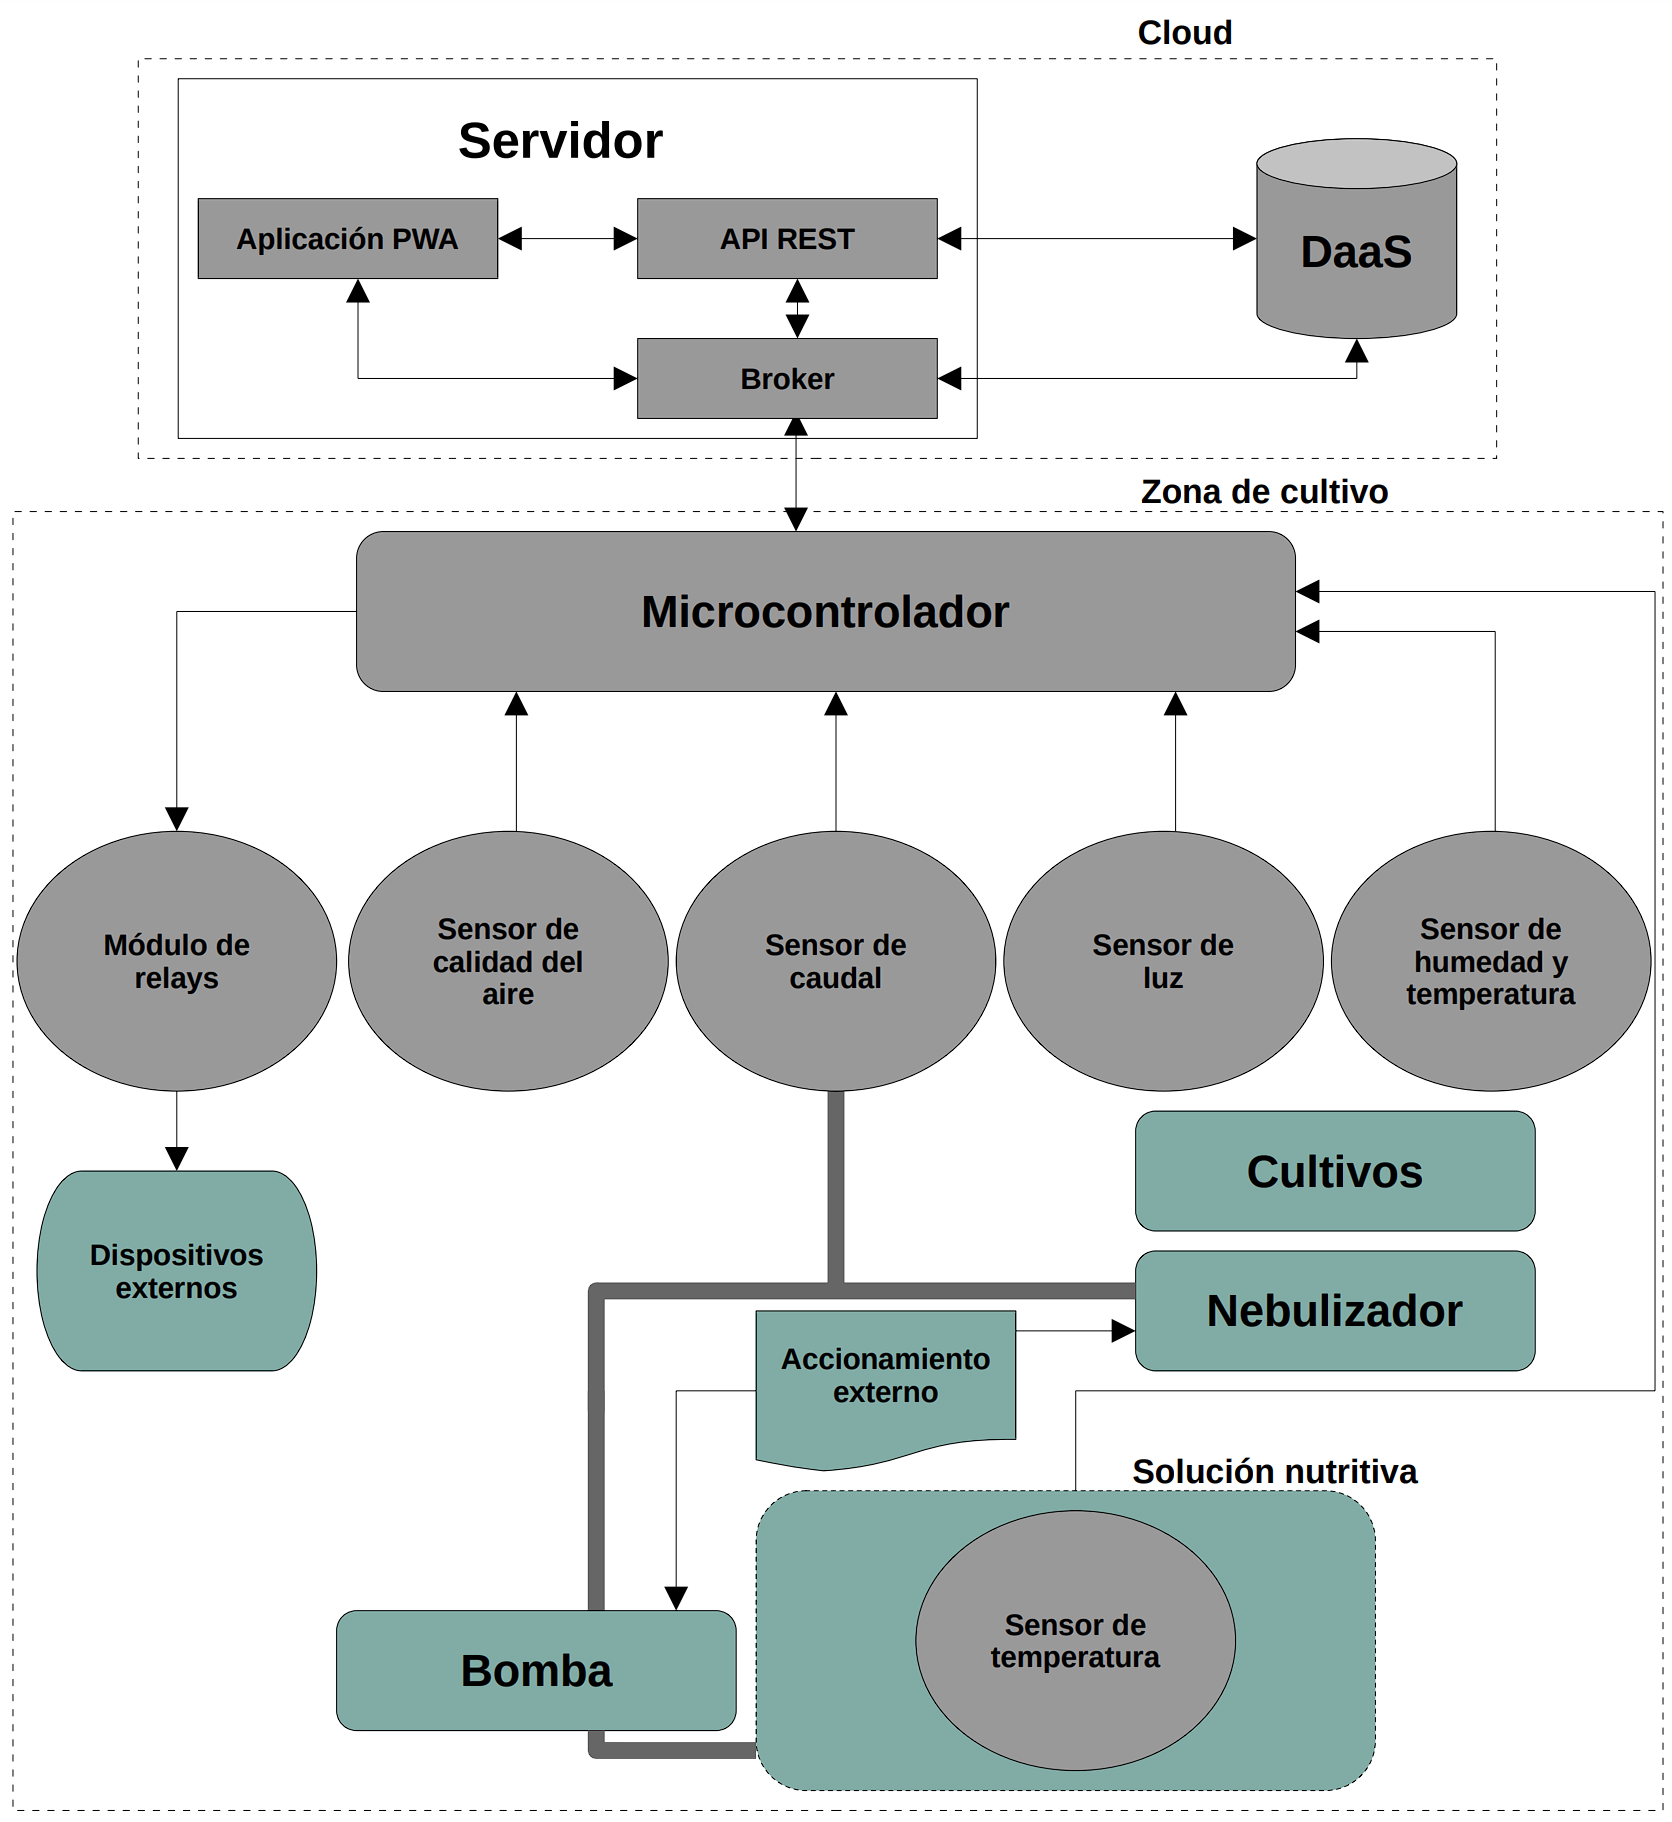
\includegraphics[width=.9\textwidth]{./Figures/Diagrama en bloques v10.png}
	\caption{Diagrama en bloques de la solución.}
	\label{fig:diagramaEnBloques}
\end{figure}

\subsection{Observaciones}
\label{sec:observaciones}

Inicialmente, en la planificación del trabajo se había planteado utilizar una aplicación SSR. Sin embargo, a la hora de comenzar el desarrollo del \textit{frontend} se decidió que una PWA sería más adecuada, ya que otorga la posibilidad de usar ciertas funcionalidades que son útiles para el sistema,  por ejemplo tener un \emph{assets cache}, utilizar notificaciones \emph{push} y permitir instalar la aplicación en los dispositivos del usuario. 

También se realizaron modificaciones en los datos a almacenar en el DaaS para cada una de las colecciones con el fin de optimizar las consultas.

Estos cambios mencionados generaron modificaciones en algunos requerimientos y tareas del trabajo.

\section{Modelo de datos}

En esta sección se describen las diferentes colecciones que se almacenan en la base de datos de MongoDB. Con el objetivo de brindar una representación visual de las mismas, se presenta su estructura por medio de las interfaces utilizadas en la API REST.

\subsection{Colección \textit{Users}}

Es la colección que contiene los datos de los usuarios. Se presenta su estructura en la figura \ref{fig:coleccionUsers}. El campo \textit{verified} sirve para indicar si el usuario verificó su \textit{email}. La propiedad \textit{passwordHash} almacena el \emph{hash} de la contraseña. El atributo \textit{pushSubscription} es un objeto embebido dentro del documento y permite enviar notificaciones \emph{push} al usuario. 

\begin{figure}[H]
	\centering
	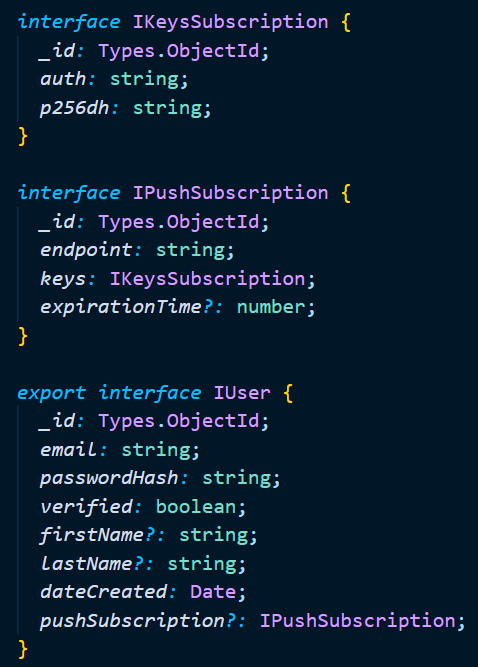
\includegraphics[width=.5\textwidth]{./Figures/Coleccion Users.png}
	\caption{Interface de la colección \textit{Users}.}
	\label{fig:coleccionUsers}
\end{figure}

\subsection{Colección \textit{Zones}}

Es la colección que contiene los datos de las zonas de cultivo. Se presenta su estructura en la figura \ref{fig:coleccionZones}. Los campos \textit{user} y \textit{lastMeasurement} son identificadores para hacer referencia a un documento de la colección \textit{Users} y \textit{Measurements}. El atributo \textit{device} es un objeto embebido dentro del documento. Este último tendrá las propiedades que indican el nombre, \emph{hash} de la contraseña, identificador de zona, identificador de usuario, alarmas asignadas junto con sus acciones automatizadas, \emph{relays} asignados y configuración de las notificaciones.

\begin{figure}[H]
	\centering
	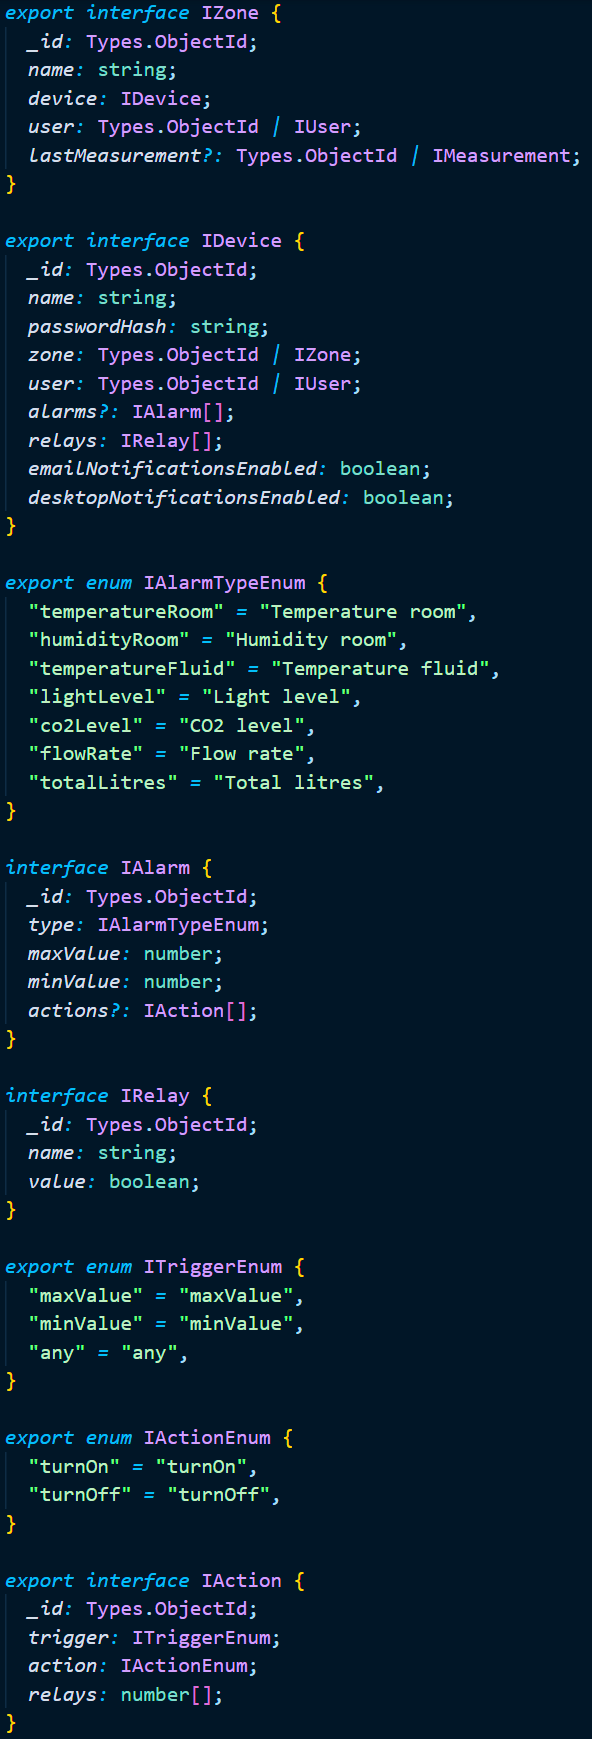
\includegraphics[width=.5\textwidth]{./Figures/Coleccion Zones.png}
	\caption{Interface de la colección \textit{Zones}.}
	\label{fig:coleccionZones}
\end{figure}

\subsection{Colección \textit{Notifications}}

Es la colección que contiene los datos de las notificaciones de los usuarios. Se presenta su estructura en la figura \ref{fig:coleccionNotifications}. Los campos \textit{zone}, \textit{device} y \textit{user} son identificadores para hacer referencia a un documento de la colección \textit{Zones}, \textit{Devices} y \textit{Users}. El atributo \textit{observation} almacena un mensaje que indica la condición que activó la alarma.

\begin{figure}[H]
	\centering
	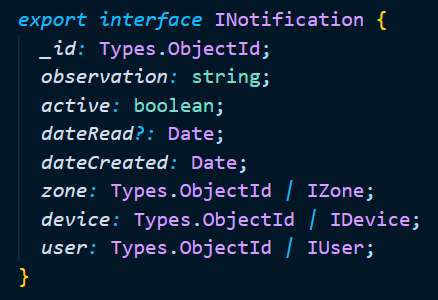
\includegraphics[width=.5\textwidth]{./Figures/Coleccion Notifications.png}
	\caption{Interface de la colección \textit{Notifications}.}
	\label{fig:coleccionNotifications}
\end{figure}

\subsection{Colección \textit{Measurements}}

Es la colección que contiene los datos de las mediciones de los sensores. Se presenta su estructura en la figura \ref{fig:coleccionMeasurements}. Las propiedades \textit{device}, \textit{zone} y \textit{user} son identificadores para hacer referencia a un documento de la colección \textit{Devices}, \textit{Zones} y \textit{Users}. El atributo \textit{timeReceived} contiene la fecha y hora de cuando se creó la medición.

\begin{figure}[H]
	\centering
	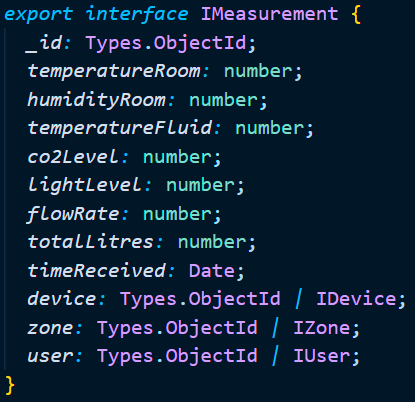
\includegraphics[width=.5\textwidth]{./Figures/Coleccion Measurements.png}
	\caption{Interface de la colección \textit{Measurements}.}
	\label{fig:coleccionMeasurements}
\end{figure}

\section{Desarrollo del \emph{backend}}

El \emph{backend} fue desarrollado en Node.js mediante TypeScript  y Express.

En el código \ref{cod:inicializacionBackend} se presenta la inicialización del \emph{backend} con certificados TLS. En las líneas 1 y 2 se obtienen los certificados. En las líneas 4 a 9 se crea el servidor con HTTPS con los certificados TLS.

\begin{lstlisting}[label=cod:inicializacionBackend,caption=Inicialización del \emph{backend} con TLS.]
const privateKey = readFileSync("./ssl/localhost.key");
const certificate = readFileSync("./ssl/localhost.crt");

const server = createServer(
   { key: privateKey, cert: certificate },
   app
).listen(port, () => {
   console.log(`[server]: Server is running at https://localhost:${port}`);
});
\end{lstlisting}

El \emph{backend} utiliza JWT (del inglés \textit{JSON Web Tokens}) para la autorización y autenticación de los usuarios. 

La autorización ocurre cuando un usuario inicia sesión en el sistema y el \emph{backend} le brinda un JWT firmado con una clave privada. En la figura \ref{fig:diagramaSecuenciaAutorizacionUsuarios} se visualiza un diagrama de secuencia del proceso.

\begin{figure}[H]
	\centering
	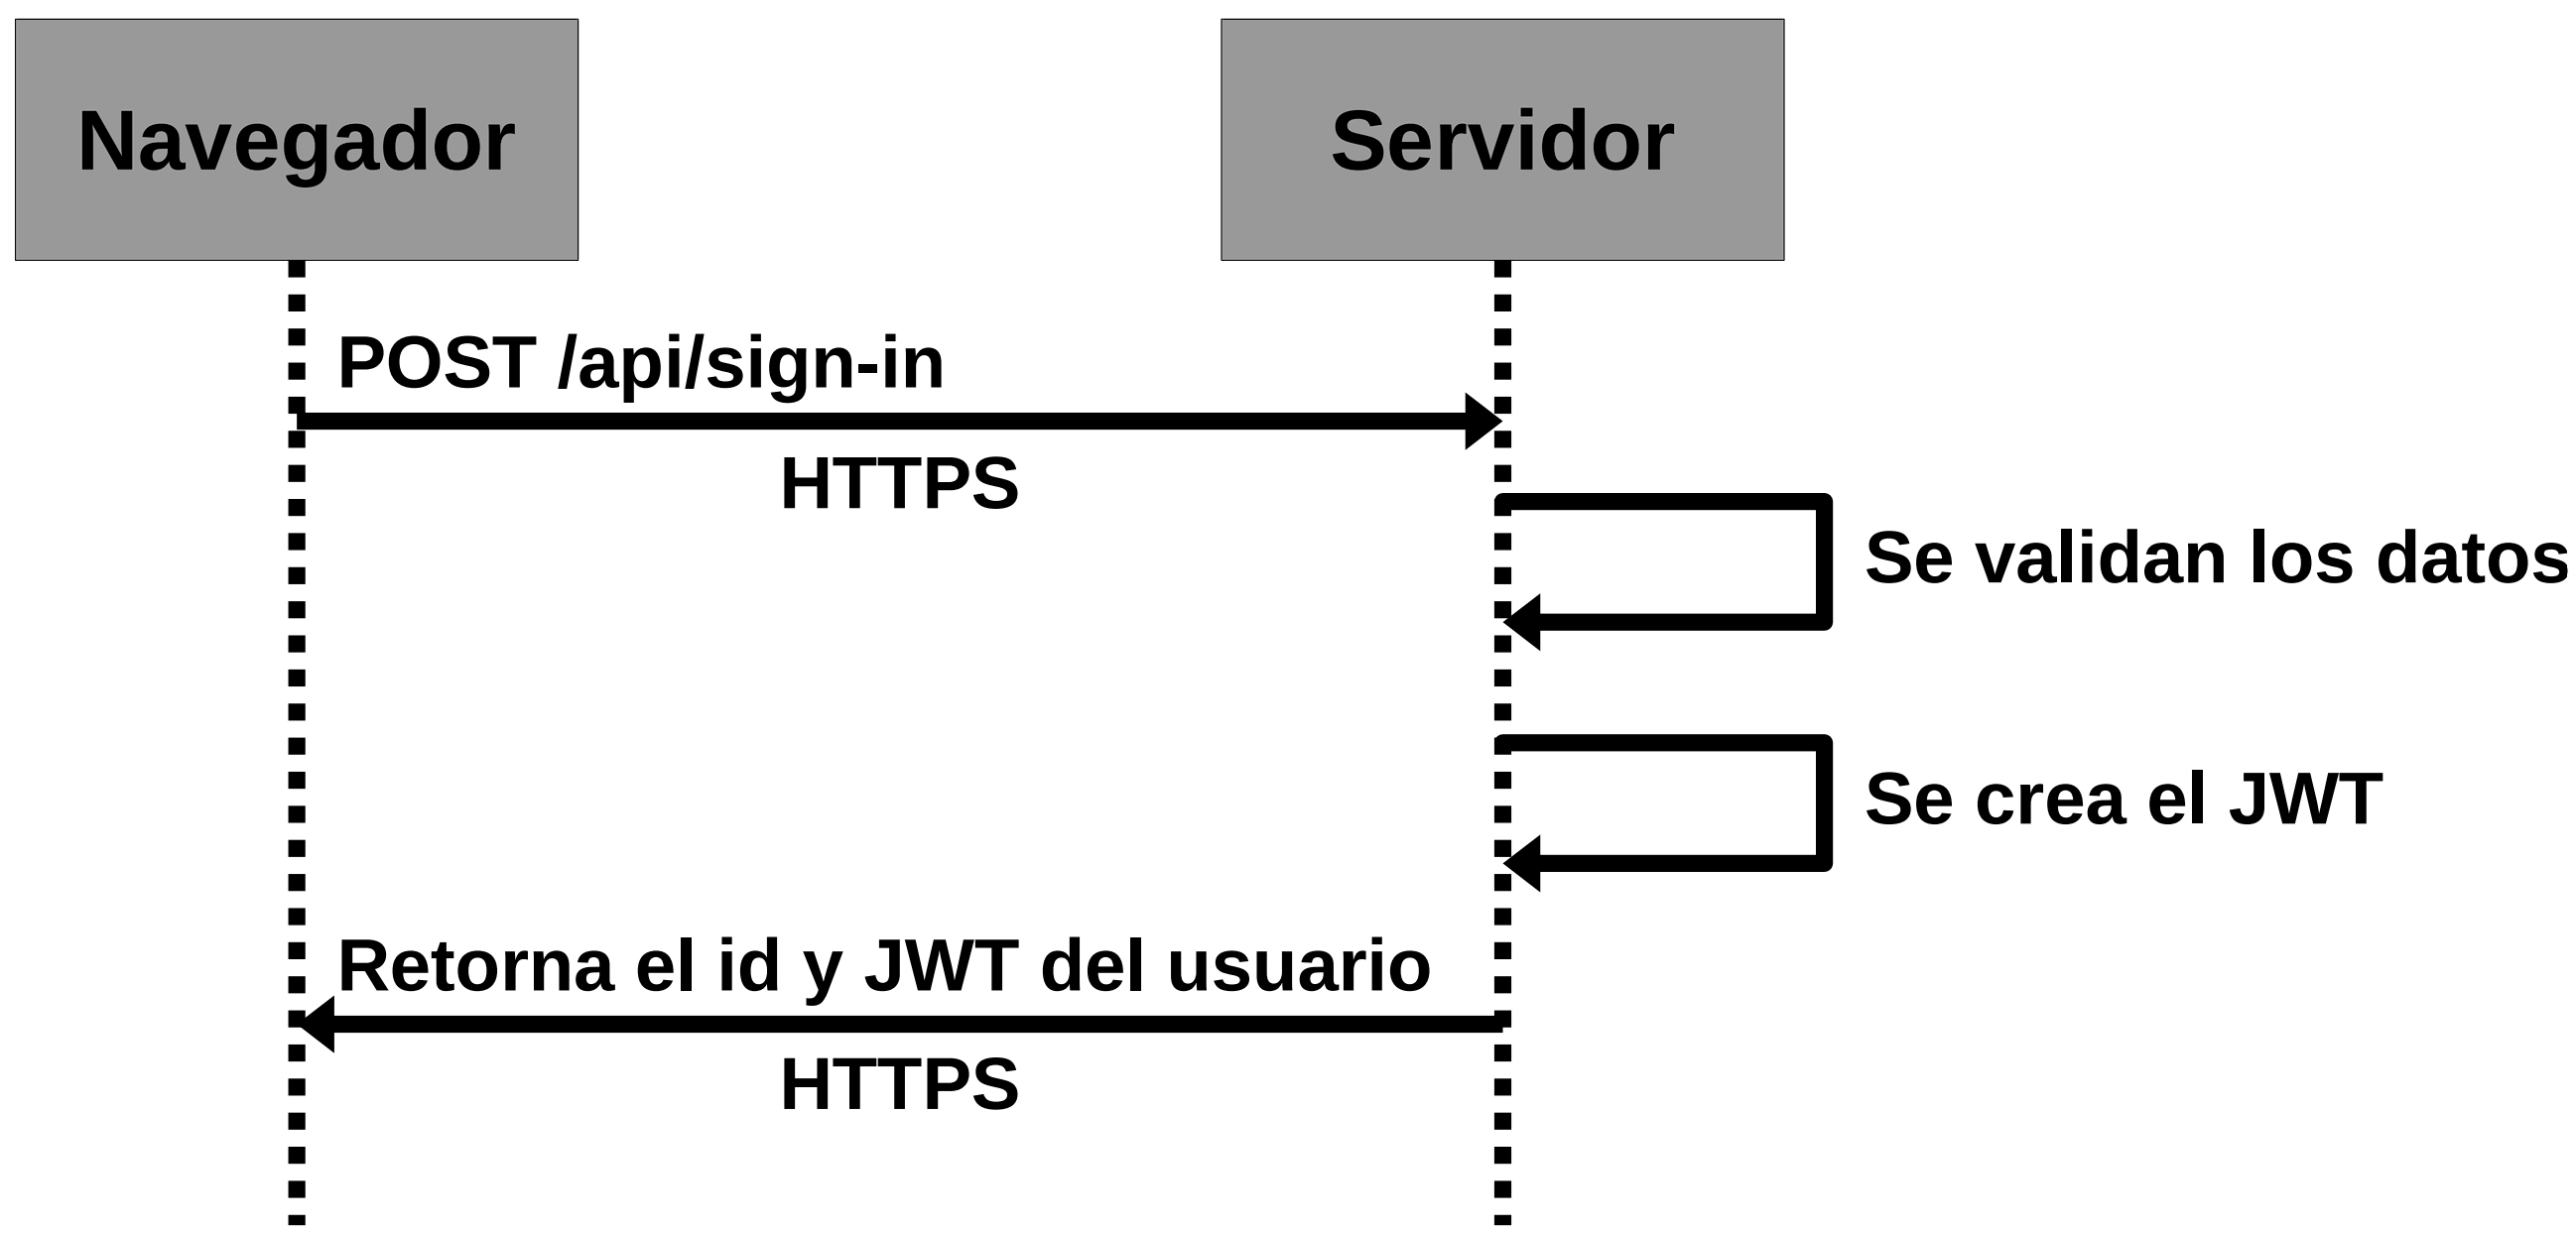
\includegraphics[width=.9\textwidth]{./Figures/Diagrama de secuencia autorizacion de usuarios.png}
	\caption{Diagrama de secuencia de la autorización de usuarios.}
	\label{fig:diagramaSecuenciaAutorizacionUsuarios}
\end{figure}

Si el usuario no dispone de credenciales válidas, la API responde con un código de error 400 y una breve descripción del error. Si se produce un error interno en el servidor, la API responde con un código de error 500.

En el código \ref{cod:autorizacionBackend} se presenta el proceso de autorización de los usuarios. En la línea 1 se obtiene la clave privada mediante las variables de entorno. En las líneas 6 a 8 se firma el \emph{payload} con la clave privada, también se asigna la expiración del JWT a siete días. En la línea 10 se le entrega al usuario el JWT junto con su id.

\begin{lstlisting}[label=cod:autorizacionBackend,caption=Autorización de usuarios.]
const accessTokenSecret = process.env["ACCESS_TOKEN_SECRET"] as string;
const payload = {
    _id: user._id,
    email: user.email,
};
const accessToken = jwt.sign(payload, accessTokenSecret, {
    expiresIn: "7d",
});

return response.status(200).json({ _id: user._id, accessToken });
\end{lstlisting} 

La autenticación ocurre cuando un usuario quiere acceder a un recurso protegido, por ejemplo un \emph{endpoint} y el \emph{backend} debe validar el JWT del usuario para determinar si puede acceder o no. En la figura \ref{fig:diagramaSecuenciaAutenticacionUsuarios} se visualiza un diagrama de secuencia del proceso.

\begin{figure}[H]
	\centering
	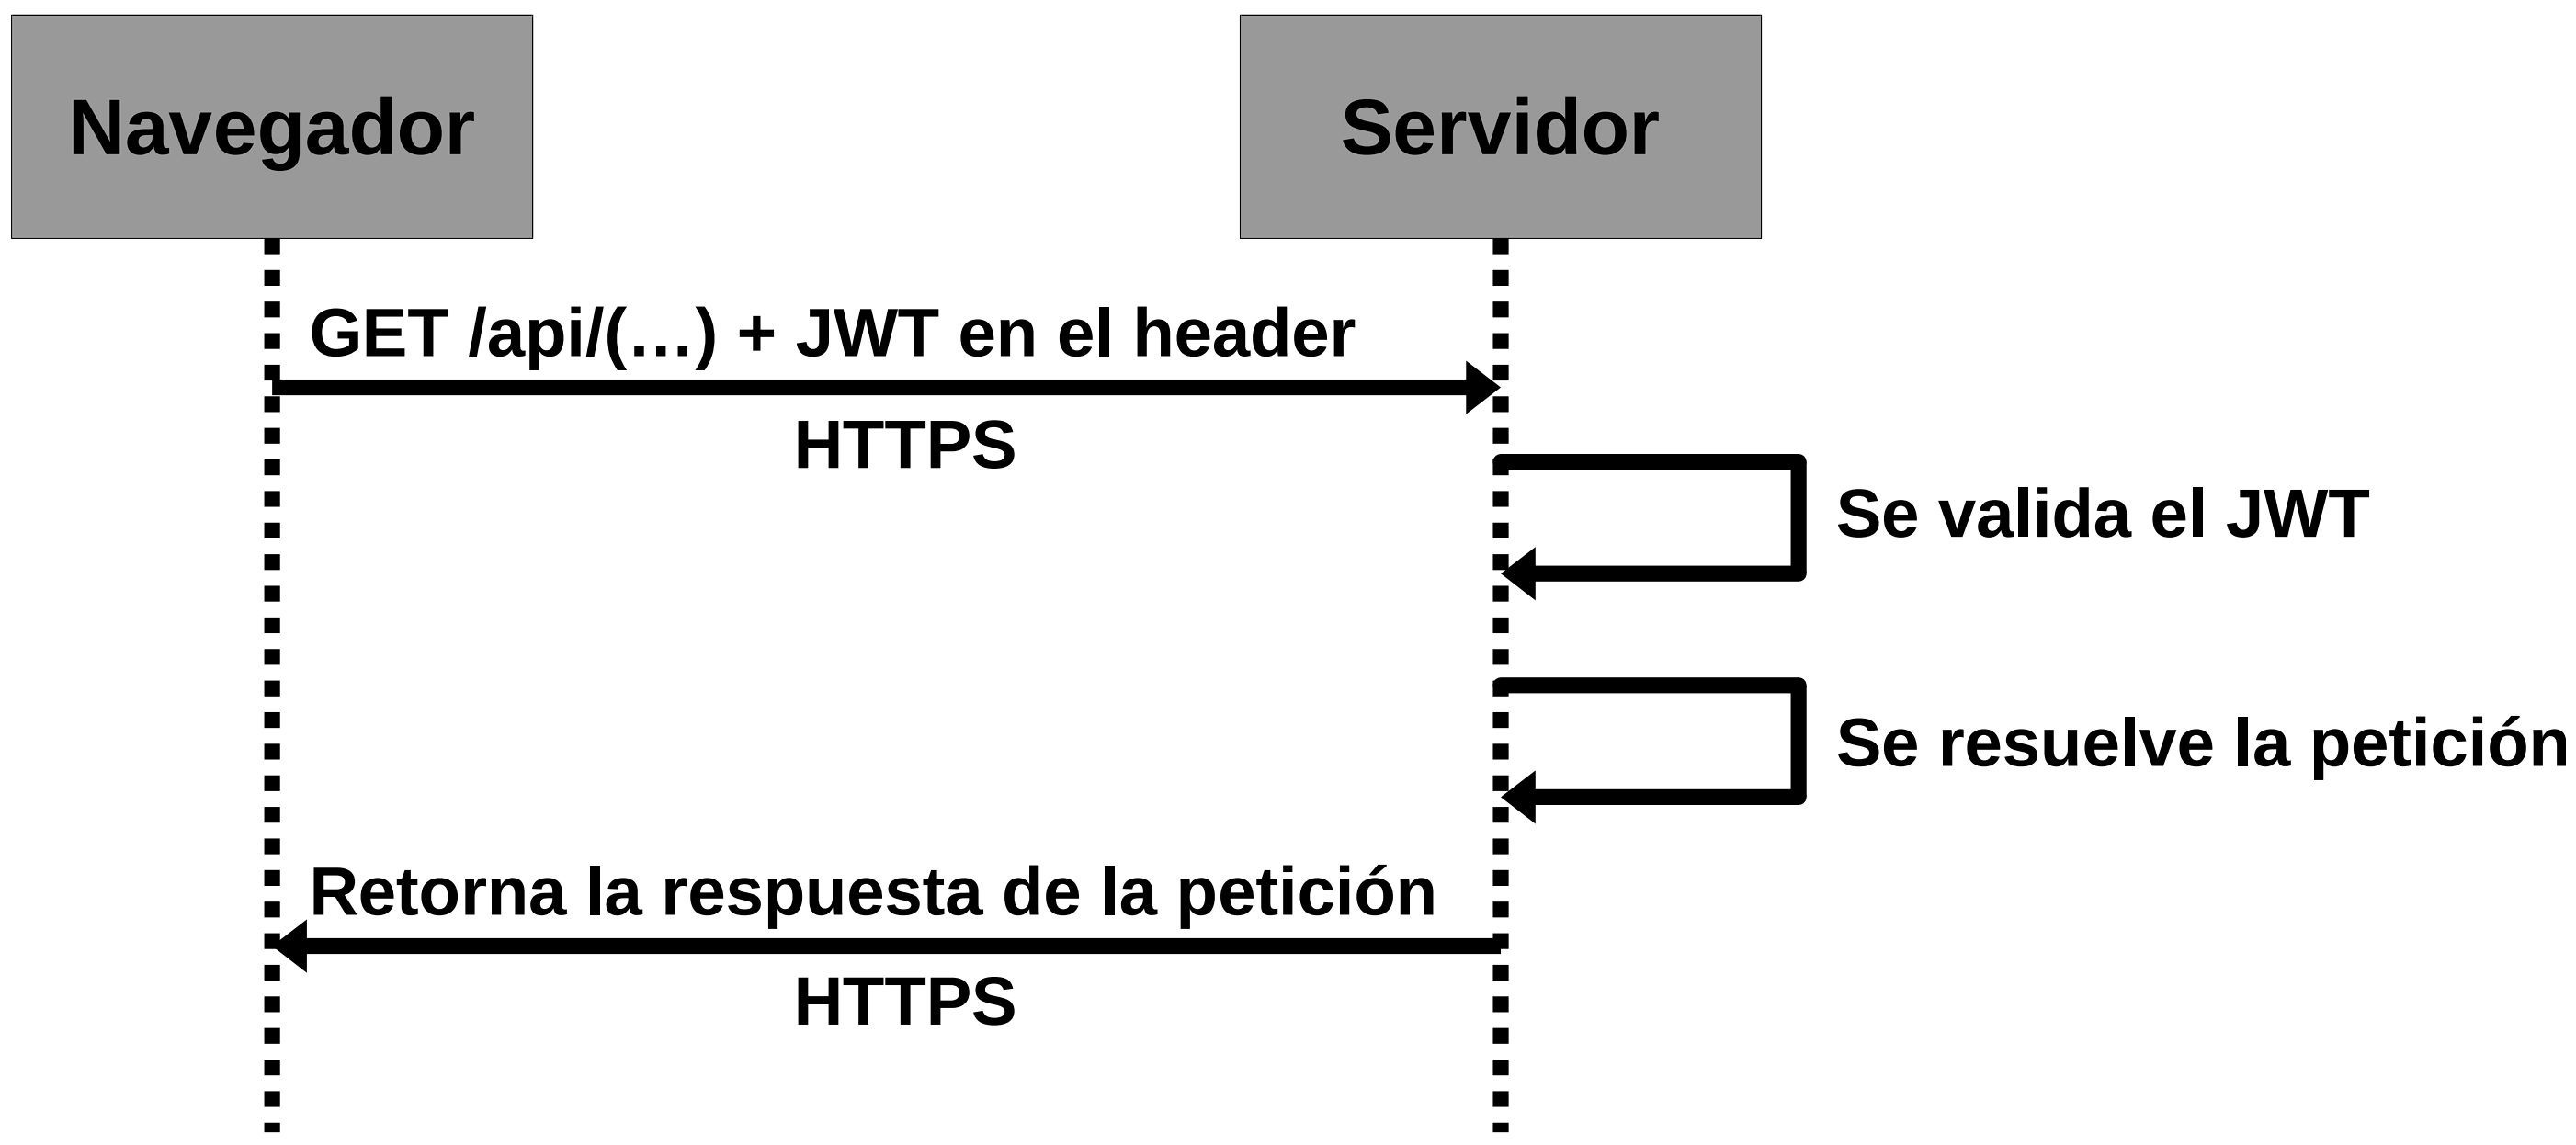
\includegraphics[width=.9\textwidth]{./Figures/Diagrama de secuencia autenticacion de usuarios.png}
	\caption{Diagrama de secuencia de la autenticación de usuarios.}
	\label{fig:diagramaSecuenciaAutenticacionUsuarios}
\end{figure}

Todos los \textit{endpoints} del sistema, excepto el de registro de usuarios y el de inicio de sesión, requieren el JWT del usuario para poder ser consultados. Si el usuario no envía el JWT, la API responde con un código de error 401. 

En el código \ref{cod:autenticaciónBackend} se presenta el proceso de autenticacion de los usuarios mediante un \emph{middleware} que protege los \emph{endpoints}. En las líneas 6 a 11 se obtiene el JWT del \textit{authorization header} \citep{WEBSITE:HTTPHEADERAUTHORIZATION} de la \emph{request} y se valida que no sea nulo. En la línea 14 se verifica el JWT mediante la biblioteca jsonwebtoken. En las líneas 15 y 16 se guarda el id e \textit{email} del usuario en la respuesta HTTP.

\begin{lstlisting}[label=cod:autenticaciónBackend,caption=Autenticación de usuarios mediante un \emph{middleware}.]
export const authorization = (
  request: Request,
  response: Response,
  next: NextFunction
) => {
  const accessToken = request.headers.authorization?.split(" ")[1];
  const accessTokenSecret = process.env["ACCESS_TOKEN_SECRET"] as string;

  if (!accessToken) {
    return response.sendStatus(401);
  }

  try {
    const payloadData = verifyToken(accessToken, accessTokenSecret);
    response.locals._id = payloadData._id;
    response.locals.email = payloadData.email;

    return next();
  } catch {
    return response.sendStatus(401);
  }
};
\end{lstlisting}

En el código \ref{cod:endpointGetZonesBackend} se presenta un ejemplo de \emph{endpoint} que requiere la autenticación del usuario. En las líneas 1 y 2 se establece el nombre de la ruta junto con el método HTTP. En la línea 3 se aplica un \emph{middleware} a la ruta que verifica el \emph{token} del usuario. En la línea 6 se obtiene su id. En las líneas 7 a 9 se utiliza el ORM (del inglés \textit{Object-Relational-Mapping}) Mongoose para obtener las zonas que le pertenecen. En la línea 10 se le entrega una lista de sus zonas.

\begin{lstlisting}[label=cod:endpointGetZonesBackend,caption=\emph{Endpoint} que requiere autenticación.]
zoneRouter.get(
  "/",
  authorization,
  async (request: Request, response: Response) => {
    try {
      const userId = response.locals._id;
      const zones = await Zone.find({ user: userId })
        .populate("lastMeasurement")
        .exec();
      return response.status(200).json(zones);
    } catch (error) {
      return response.status(500).json(error);
    }
  }
);
\end{lstlisting} 

En la tabla \ref{tab:tablaEndpointsBackend} se pueden observar los \textit{endpoints} disponibles.

\begin{table}[H]
	\centering
	\caption[\textit{Endpoints} disponibles]{\textit{Endpoints} disponibles.}
	\begin{tabular}{l c c}    
		\toprule
		\textbf{\emph{Endpoint}} & \textbf{Método} & \textbf{Descripción}\\
		\midrule
		/auth/sign-up & \emph{POST} & \shortstack{Permite registrar un  \\ usuario} \\
		/auth/sign-in & \emph{POST} & Permite iniciar sesión \\
		/auth/verifyToken & \emph{GET} & Permite verificar al usuario \\
		/auth/profile & \emph{GET} & \shortstack{Permite obtener los \\ datos del usuario} \\
		/auth/profile & \emph{PATCH} & \shortstack{Permite actualizar los \\ datos del usuario} \\
		/notifications & \emph{GET} & \shortstack{Permite obtener las \\ notificaciones} \\
		/notifications/markAsRead/:id & \emph{PATCH} & \shortstack{Permite marcar una \\ notificación como leída } \\
		/notifications/subscribe & \emph{PATCH} & \shortstack{Permite suscribirse a \\ las notificaciones } \\
		/measurements/zones/id: & \emph{POST} & \shortstack{Permite simular una \\ medición en una zona} \\
		/measurements/zones/:id & \emph{GET} &  \shortstack{Permite obtener las \\ mediciones de una zona } \\
		/zones & \emph{GET} & \shortstack{Permite obtener las zonas } \\
		/zones/:id & \emph{GET} & Permite obtener una zona \\
		/zones & \emph{POST} & Permite crear una zona \\
		/zones & \emph{PATCH} & \shortstack{Permite actualizar los \\  datos de una zona } \\
		/zones/:id & \emph{DELETE} & Permite eliminar una zona \\
		/zones/relays/:id & \emph{PATCH} & \shortstack{Permite actualizar los \\  datos de un \emph{relay} } \\
		\bottomrule
		\hline
	\end{tabular}
	\label{tab:tablaEndpointsBackend}
\end{table}

En la figura \ref{fig:estructuraDeDirectoriosDelBackend} se presenta la estructura de directorios. La descripción de los contenidos de las carpetas y archivos relevantes es:
\begin{itemize}
	\item models: contiene las interfaces que permiten al ORM Mongoose tipificar las colecciones de MongoDB.
	\item routes: contiene los \emph{endpoints}.
	\item schemas: contiene los esquemas que permiten al ORM Mongoose crear las colecciones en MongoDB.
	\item ssl: contiene los certificados TLS.
	\item utils: contiene un \emph{middleware} para autorizar los \emph{endpoints} necesarios. Además, contiene funciones que se reutilizan en todo el proyecto.
	\item .env: contiene las variables de entorno.
	\item broker.ts: contiene la inicialización y configuración del \emph{broker} Aedes.
	\item index.ts: contiene la inicialización y configuración del \emph{backend}.
	\item jest.config.js: contiene la configuración de Jest.
	\item ts.config.json: contiene la configuración de TypeScript.
\end{itemize}

\begin{figure}[H]
	\centering
	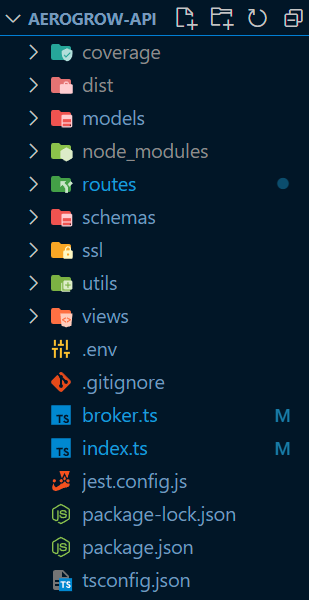
\includegraphics[width=.4\textwidth]{./Figures/Estructura de directorios del backend.png}
	\caption{Estructura de directorios.}
	\label{fig:estructuraDeDirectoriosDelBackend}
\end{figure}

\section{Desarrollo del \emph{frontend}}
El \emph{frontend} del trabajo fue desarrollado en TypeScript con Angular y como \textit{framework} de estilos se utilizó Angular Material.

La estrategia de diseño que se utilizó fue la de crear una PWA con un enfoque de diseño \emph{responsive} \citep{WEBSITE:RESPONSIVE}.

Para obtener el mejor rendimiento posible en la aplicación se aplicaron diferentes estrategias de optimización \citep{WEBSITE:ANGULAROPTIMIZACION1} \citep{WEBSITE:ANGULAROPTIMIZACION2}, entre ellas destacan las siguientes:
\begin{itemize}
	\item \emph{Lazy loading} de rutas.
	\item \emph{Lazy loading} de imágenes.
	\item Uso de \textit{ChangeDetectionStrategy.onPush} en los componentes.
	\item \textit{Assets cache}.
	\item Evitar llamadas de funciones en las vistas HTML.
	\item Utilizar el \emph{guard} canLoad.
	\item Evitar el uso de bibliotecas que no sean esenciales para el trabajo.
	\item Evitar suscripciones manuales a un \textit{Observable} \citep{WEBSITE:OBSERVABLE}. 
\end{itemize}

En la figura \ref{fig:certificadosTLSDelFrontend} se presenta la configuración para utilizar certificados TLS.

\begin{figure}[H]
	\centering
	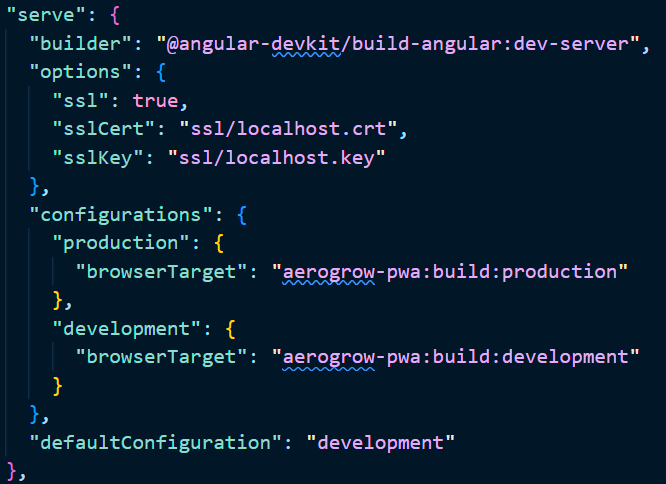
\includegraphics[width=.6\textwidth]{./Figures/Certificados TLS en Angular.png}
	\caption{Uso de certificados TLS.}
	\label{fig:certificadosTLSDelFrontend}
\end{figure}

La PWA utiliza un \emph{guard} para la autenticación de las rutas.  En el código \ref{cod:autenticaciónFrontend} se presenta el proceso de autenticación de las rutas. En la línea 7 se obtiene el estado de la sesión del usuario. En las líneas 9 a 13 se verifica su estado: si inició sesión puede entrar a la ruta, caso contrario se le redirecciona a la pantalla del \emph{login}.

\begin{lstlisting}[label=cod:autenticaciónFrontend,caption=Autenticación de rutas.]
export const authGuard = (
  route: ActivatedRouteSnapshot,
  state: RouterStateSnapshot
) => {
  const router = inject(Router);
  const authService = inject(AuthService);
  const isLoggedIn = authService.isLoggedIn();

  return isLoggedIn
    ? true
    : router.navigate(['/sign-in'], {
        queryParams: { returnUrl: state.url },
      });
};
\end{lstlisting} 

En la tabla \ref{tab:tablaRutasFrontend} se pueden observar las rutas disponibles.

\begin{table}[H]
	\centering
	\caption[Rutas disponibles]{Rutas disponibles.}
	\begin{tabular}{l c c}    
		\toprule
		\textbf{Ruta}& \textbf{Descripción}\\
		\midrule
		/ & Pantalla de listado de zonas \\
		/profile & Pantalla de edición de un usuario \\
		/zones & Pantalla de listado de zonas \\
		/zones/create & Pantalla de creación de una zona \\
		/zones/edit/:id & Pantalla de edición de una zona \\
		/notifications & Pantalla de listado de notificaciones \\
		/dashboard/:id & Pantalla de \emph{dashboard} de una zona \\
		/sign-in & Pantalla de inicio de sesión \\
		/sign-up & Pantalla de registro de usuario \\
		/error/:code & Pantalla de manejo de errores \\
		\bottomrule
		\hline
	\end{tabular}
	\label{tab:tablaRutasFrontend}
\end{table}

En la figura \ref{fig:estructuraDeDirectoriosDelFrontend} se presenta la estructura de directorios. La descripción de los contenidos de las carpetas y archivos relevantes es:
\begin{itemize}
	\item src/app/components: contiene los componentes del proyecto.
	\item src/app/guards: contiene un \emph{guard} para autenticar las rutas.
	\item src/app/interceptors: contiene un \textit{interceptor} que añade el JWT del usuario al \textit{header} de la \emph{request} y gestiona los errores de las \emph{requests} HTTP.
	\item src/app/models: contiene las interfaces para tipificar los datos del sistema.
	\item src/app/services: contiene los servicios del proyecto.
	\item src/app/utils: contiene funciones que se reutilizan en todo el proyecto.
	\item src/app/app.component.ts: contiene el componente con el que se inicializa la aplicación.  
	\item src/app/routes.ts: contiene las rutas de la aplicación.
	\item src/assets: contiene los \emph{assets} del \emph{frontend}.
	\item src/manifest.webmanifest: contiene el archivo de manifiesto del proyecto.
	\item src/robots.txt: contiene la configuración para los \emph{crawlers} \citep{WEBSITE:CRAWLER}.
	\item angular.json: contiene la configuración de Angular.
	\item bs-config.js: contiene la configuración de lite-server. 
	\item karma.config: contiene la configuración de Jasmine y Karma \citep{WEBSITE:KARMA} para las pruebas.
	\item ngsw-config: contiene la configuración del \emph{service worker} de la PWA.
	\item ts.config.json: contiene la configuración de TypeScript.
\end{itemize}

\begin{figure}[H]
	\centering
	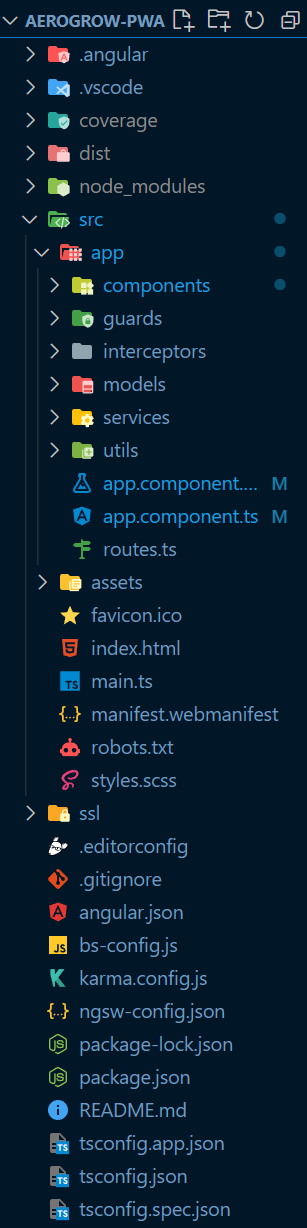
\includegraphics[width=.3\textwidth]{./Figures/Estructura de directorios del frontend.png}
	\caption{Estructura de directorios.}
	\label{fig:estructuraDeDirectoriosDelFrontend}
\end{figure}

\subsection{Principales pantallas de la aplicación}

En la figura \ref{fig:formularioSignUp} se visualiza la pantalla de creación de usuarios. Para dar de alta un nuevo usuario se debe ingresar de forma mandatoria su  \textit{email} y contraseña, de forma opcional se puede agregar el nombre y apellido. Las cuentas tienen un lapso de 10 días para confirmarse mediante \textit{email} antes de ser eliminadas.

\begin{figure}[H]
	\centering
	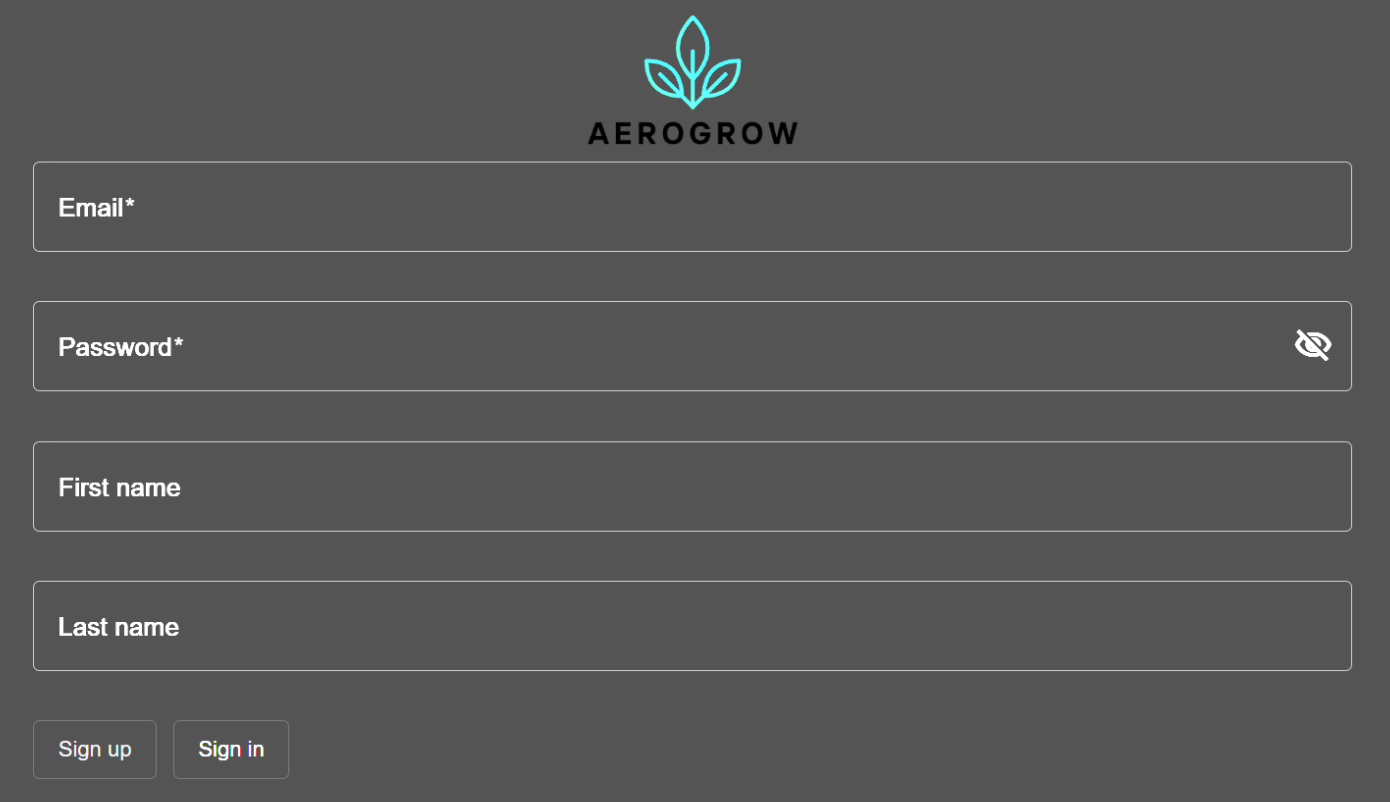
\includegraphics[width=.8\textwidth]{./Figures/Frontend formulario de creacion de nueva cuenta.png}
	\caption{Pantalla de registro de usuario.}
	\label{fig:formularioSignUp}
\end{figure}

En la figura \ref{fig:listaDeZonas} se visualiza la pantalla del listado de zonas de un usuario. Desde esta pantalla, puede realizar las siguientes acciones:

\begin{itemize}
	\item Acceder a una pantalla para crear una nueva zona.
	\item Acceder a una pantalla para editar una zona.
	\item Acceder a una pantalla \emph{dashboard} de una zona.
	\item Eliminar una zona.
	\item Monitorear en tiempo real todas las zonas listadas.
	\item Exportar los datos del listado en formato xlsx.
	\item Copiar las credenciales de una zona.
\end{itemize}

El listado de zonas se puede filtrar y ordenar por cualquiera de los campos de la tabla.

\begin{figure}[H]
	\centering
	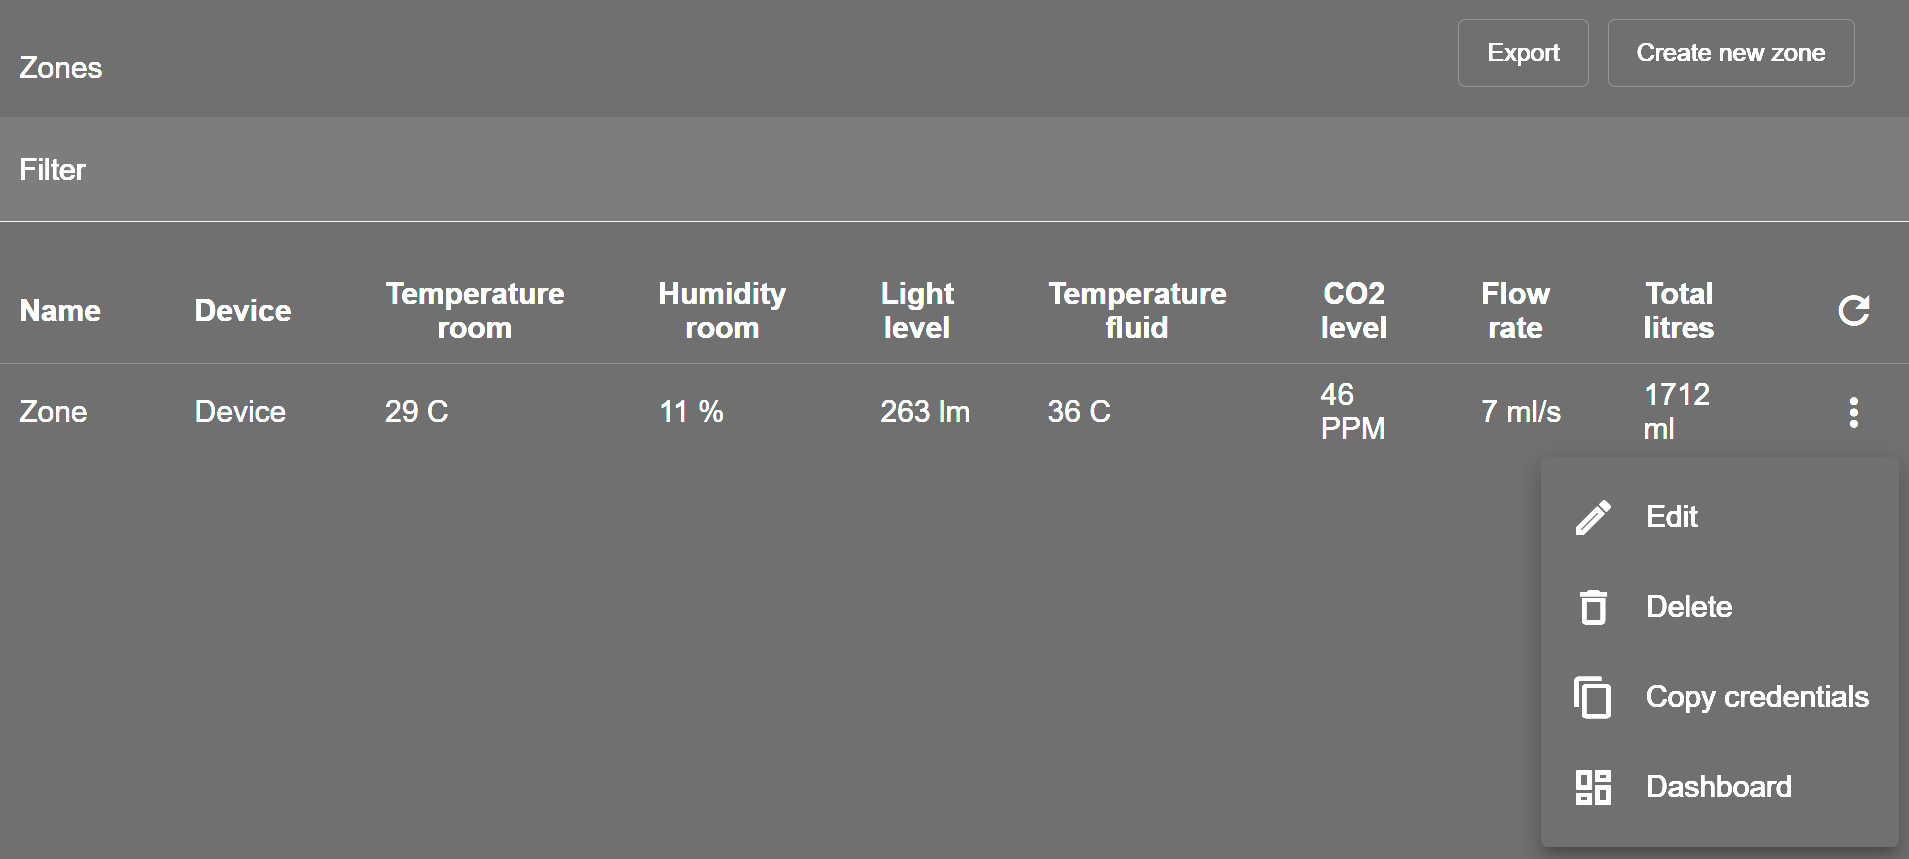
\includegraphics[width=.9\textwidth]{./Figures/Frontend lista de zonas.png}
	\caption{Pantalla de listado de zonas.}
	\label{fig:listaDeZonas}
\end{figure}

En la figura \ref{fig:formularioDeZona} se visualiza la pantalla de creación de zonas. Para crear una nueva zona se debe ingresar un nombre y también el nombre y contraseña del dispositivo. De manera opcional, se puede ingresar la configuración para las notificaciones, los \textit{relays} y alarmas asociadas al dispositivo y las acciones automatizadas a realizar en caso de que la alarma se dispare. El mismo componente es utilizado para la edición de zonas. 

\begin{figure}[H]
	\centering
	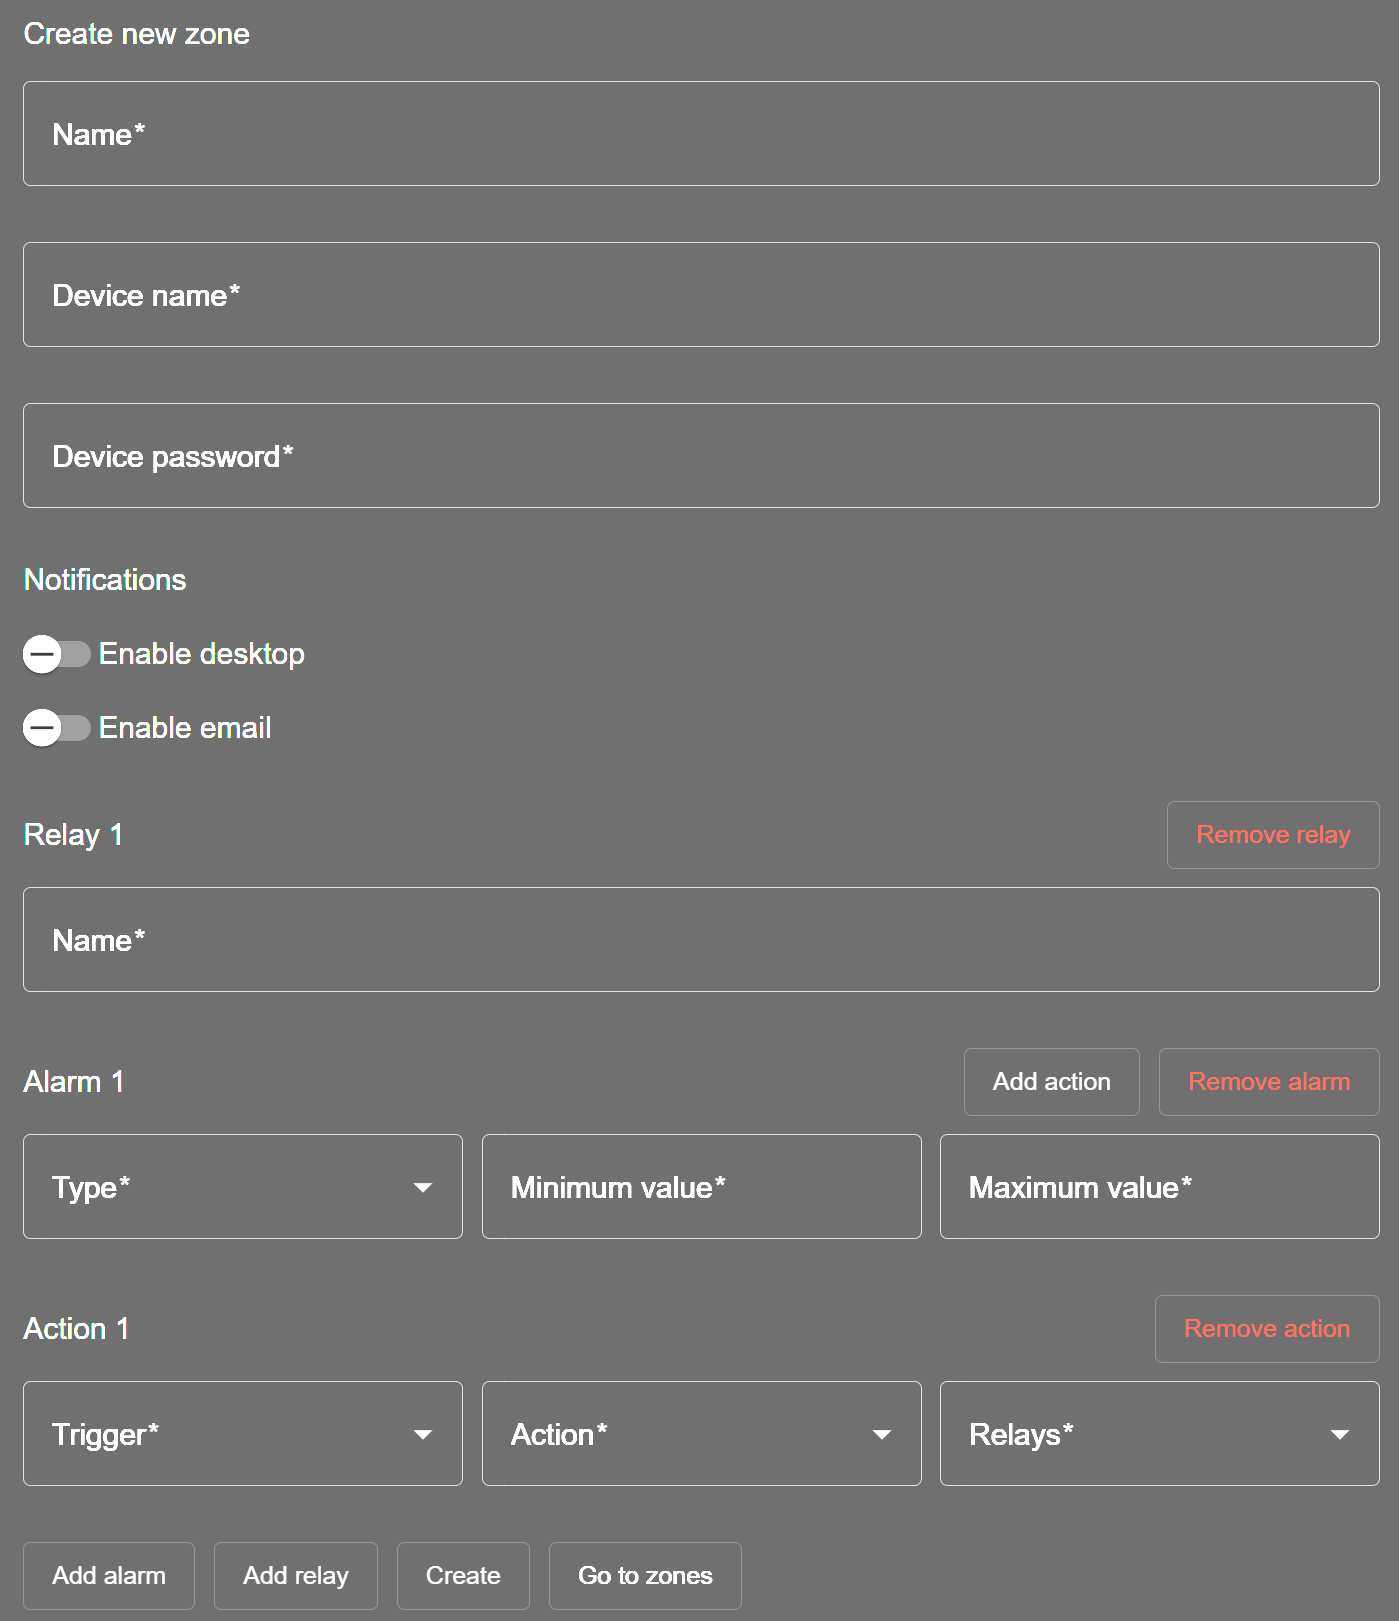
\includegraphics[width=.7\textwidth]{./Figures/Frontend formulario de zona.png}
	\caption{Pantalla de creación de una zona.}
	\label{fig:formularioDeZona}
\end{figure}

En la figura \ref{fig:notificacionAlarmaEmail} se visualiza un ejemplo de \textit{email} de notificación que envía el sistema. Este tipo de notificación se genera cuando una medición activa una alarma y las notificaciones de \textit{email} están habilitadas en la zona de cultivo.

\begin{figure}[H]
	\centering
	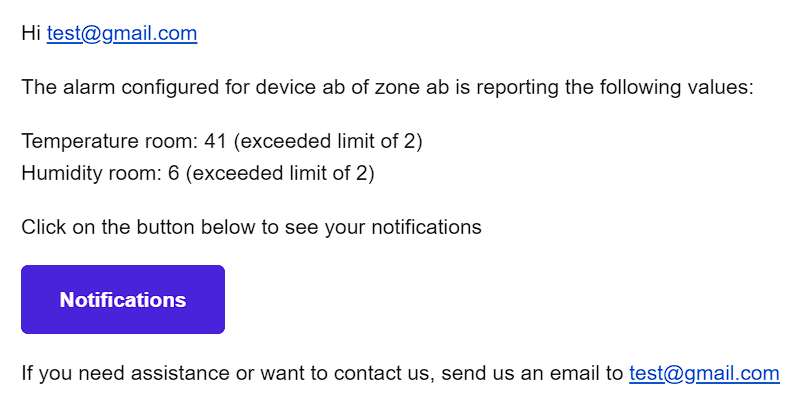
\includegraphics[width=.9\textwidth]{./Figures/Notificacion email.png}
	\caption{Ejemplo de \textit{email} de notificación de alarma.}
	\label{fig:notificacionAlarmaEmail}
\end{figure}

En la figura \ref{fig:notificacionPushEmail} se visualiza un ejemplo de notificación \emph{push} que envía el sistema. Este tipo de notificación se genera cuando una medición activa una alarma y las notificaciones de escritorio están habilitadas en la zona de cultivo.

\begin{figure}[H]
	\centering
	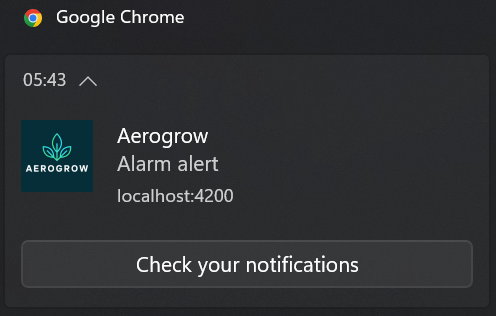
\includegraphics[width=.6\textwidth]{./Figures/Notificacion push.png}
	\caption{Ejemplo de notificacion \emph{push}.}
	\label{fig:notificacionPushEmail}
\end{figure}

En la figura \ref{fig:listaDeNotificaciones} se visualiza la pantalla del listado de notificaciones de un usuario. El listado se actualiza en tiempo real y se puede filtrar por período de tiempo y por cualquier campo de la tabla. Además, el usuario puede exportar los datos en formato xlsx y marcar las notificaciones como leídas.

\begin{figure}[H]
	\centering
	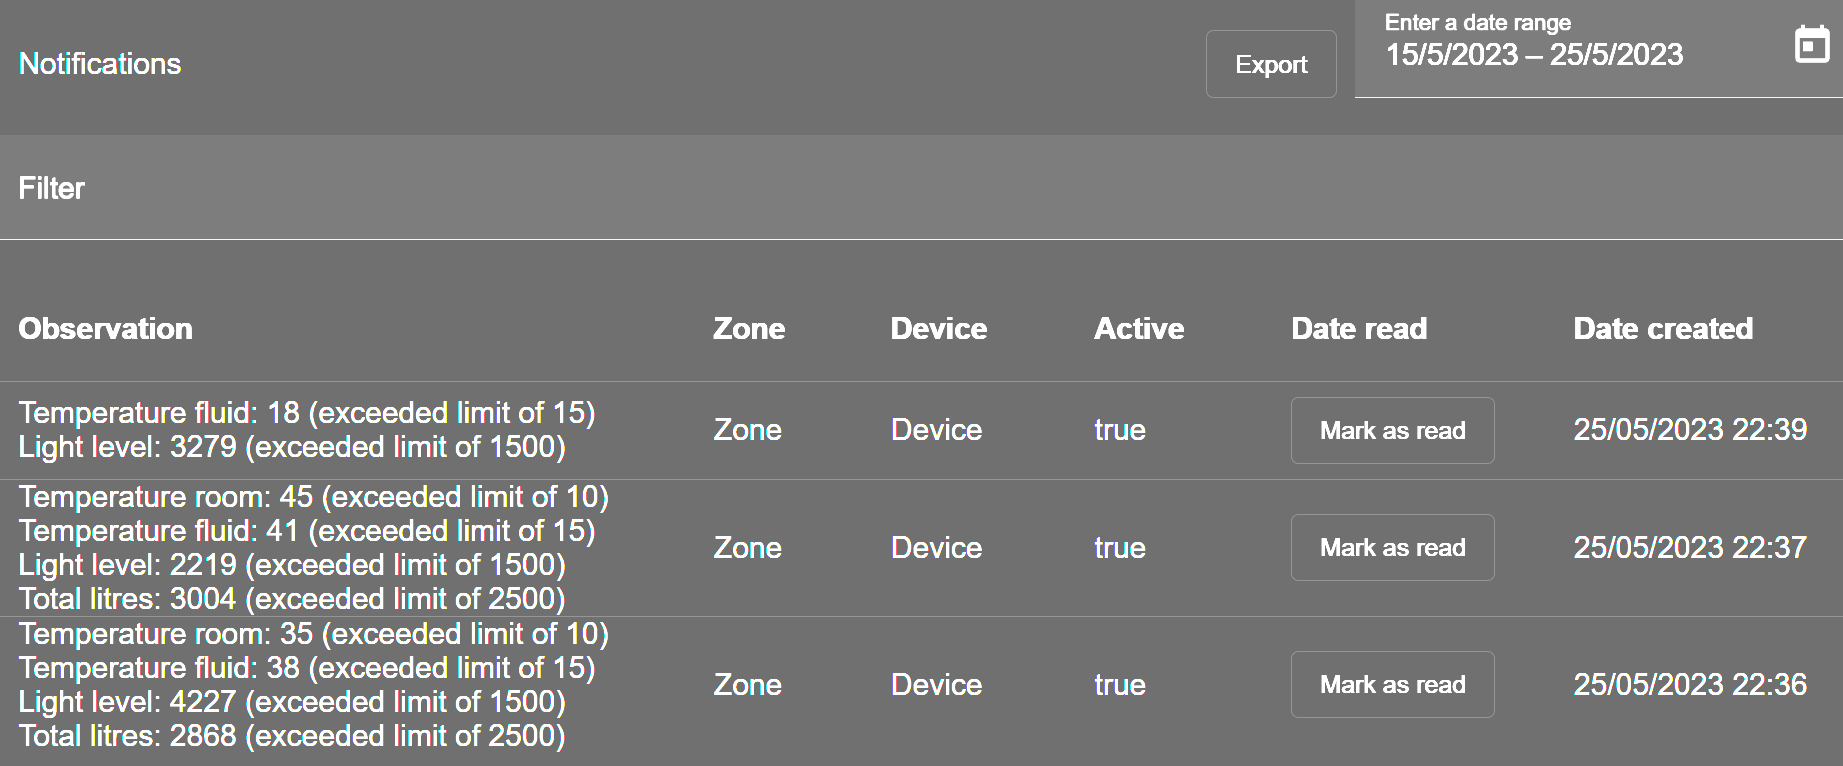
\includegraphics[width=.9\textwidth]{./Figures/Frontend lista de notificaciones.png}
	\caption{Pantalla de listado de notificaciones.}
	\label{fig:listaDeNotificaciones}
\end{figure}

En las figuras \ref{fig:tablaMedicionesDashboardDeZona}, \ref{fig:graficoMedicionesDashboardDeZona} y \ref{fig:cardsDashboardDeZona} se presentan los componentes que forman la pantalla de \emph{dashboard} de una zona. 

En la figura \ref{fig:tablaMedicionesDashboardDeZona} se visualiza el listado de mediciones de una zona. El listado se actualiza en tiempo real y se puede filtrar por período de tiempo y por cualquier campo de la tabla. Además, el usuario puede exportar los datos en formato xlsx.

\begin{figure}[H]
	\centering
	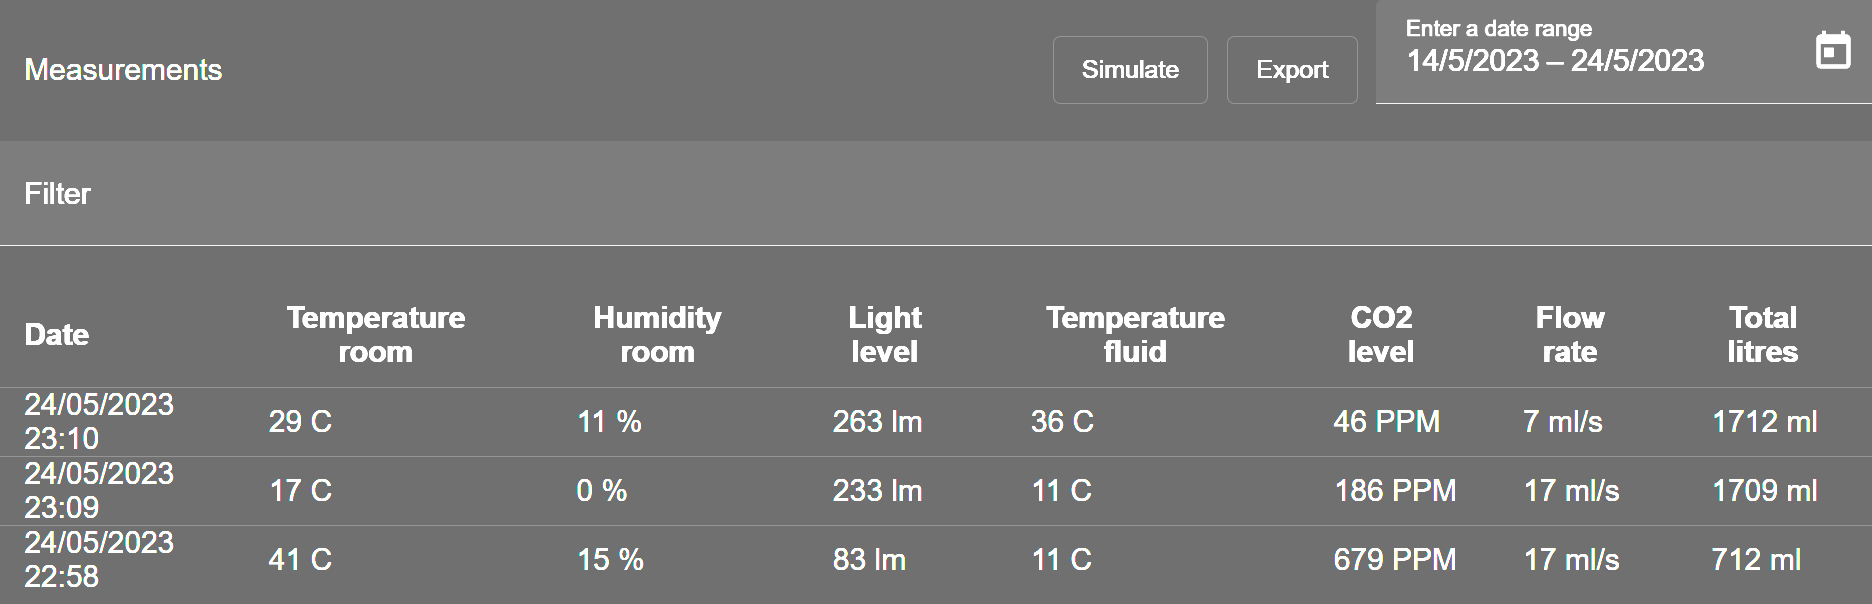
\includegraphics[width=.9\textwidth]{./Figures/Frontend dashboard de zona tabla.png}
	\caption{Listado de mediciones en vista de \textit{dashboard}.}
	\label{fig:tablaMedicionesDashboardDeZona}
\end{figure}

En la figura \ref{fig:graficoMedicionesDashboardDeZona} se visualiza el gráfico de las mediciones recibidas en el período de tiempo seleccionado. El componente permite seleccionar el tipo de atributo que se quiere graficar y se actualiza en tiempo real.

\begin{figure}[H]
	\centering
	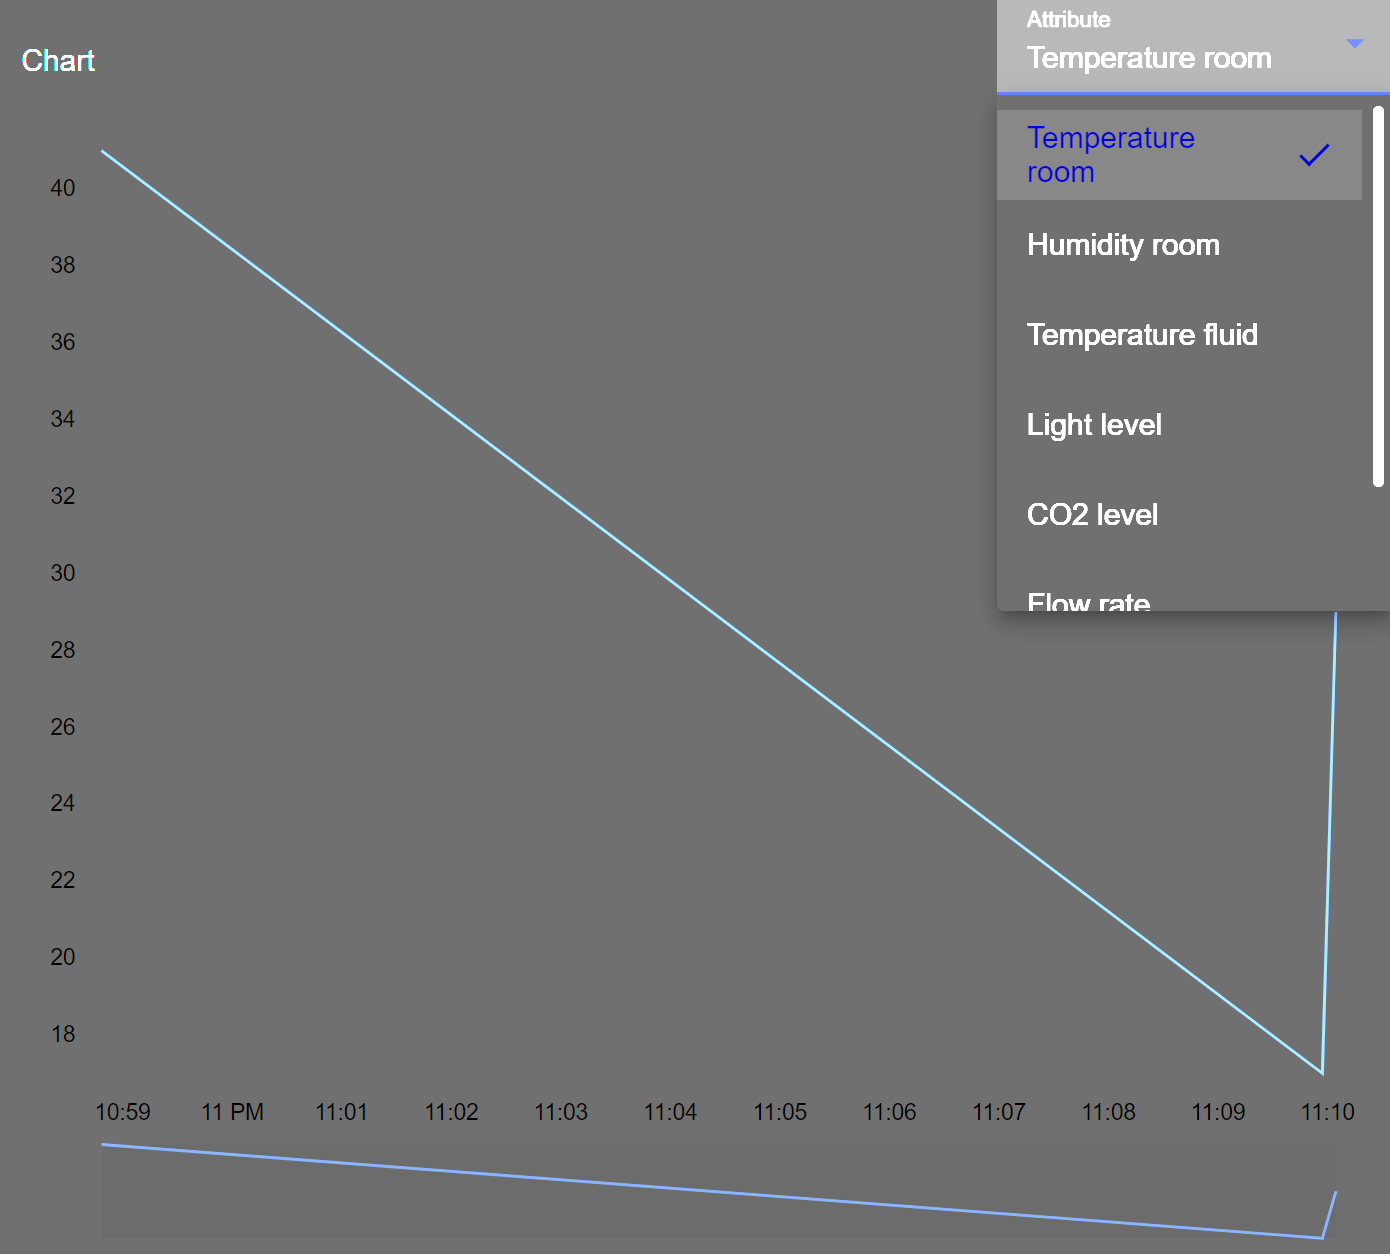
\includegraphics[width=.7\textwidth]{./Figures/Frontend dashboard de zona grafico.png}
	\caption{Gráfico de mediciones en vista de \textit{dashboard}.}
	\label{fig:graficoMedicionesDashboardDeZona}
\end{figure}

En la figura \ref{fig:cardsDashboardDeZona} se presentan las \emph{cards} del \emph{dashboard}. Las \textit{cards} se actualizan en tiempo real y permiten monitorear los datos de la última medición y accionar los \textit{relays} de la zona. 

\begin{figure}[H]
	\centering
	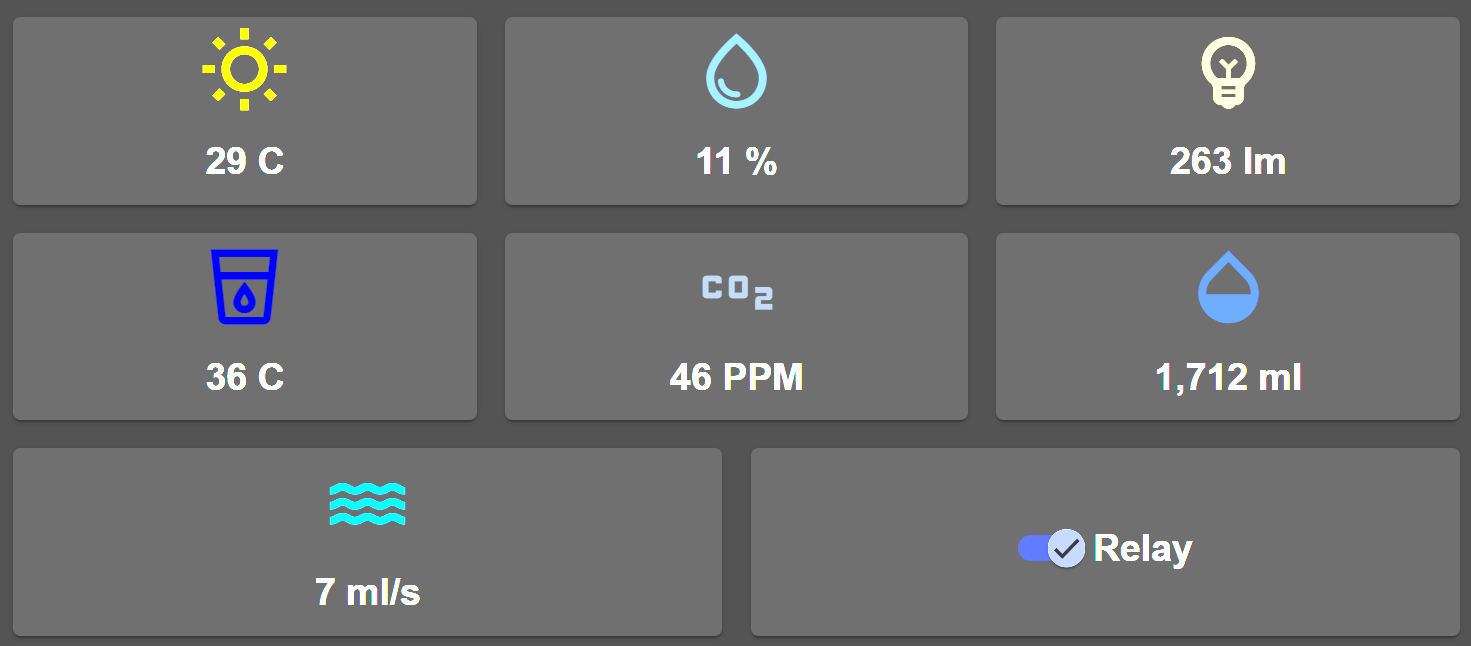
\includegraphics[width=.7\textwidth]{./Figures/Frontend dashboard de zona cards.png}
	\caption{\textit{Cards} en vista de \textit{dashboard}.}
	\label{fig:cardsDashboardDeZona}
\end{figure}

\section{Desarrollo del \emph{broker}}

El \emph{broker} fue desarrollado en Node.js mediante TypeScript y Aedes.

En el código \ref{cod:inicializacionBroker} se presenta la inicialización del \emph{broker} con certificados TLS. En las líneas 1 a 3 se obtienen los certificados. En las líneas 5 a 11 se configuran las opciones del \emph{broker}: se asignan los certificados, se solicita a los clientes que tengan certificados válidos  y se rechazan las conexiones que no tengan una autoridad de certificación \citep{WEBSITE:AUTORIDADDECERTIFICACION} válida. En la línea 12 se establece el número de puerto que utiliza el \emph{broker}. En las líneas 13 a 19 se crea el \emph{broker} con las opciones configuradas.

\begin{lstlisting}[label=cod:inicializacionBroker,caption=Inicialización del \emph{broker} con TLS.]
const ca = readFileSync("ssl/ca.crt");
const privateKey = readFileSync("./ssl/broker.key");
const certificate = readFileSync("./ssl/broker.crt");

const options: TlsOptions = {
   key: privateKey,
   cert: certificate,
   ca: ca,
   requestCert: true,
   rejectUnauthorized: true,
};
const mqttPort = 8883;
const mqttServer = createServer(options, aedes.handle);

mqttServer.listen(mqttPort, () => {
   console.log(
     `[server]: MQTT Server is running at mqtts://localhost:${mqttPort}`
   );
});
\end{lstlisting}

El \emph{broker} utiliza como medida extra de seguridad un proceso de autenticación mediante usuario y contraseña. En el código \ref{cod:autenticaciónBroker} se presenta el proceso de autenticación de los clientes. En las líneas 7 a 12 se verifica que el usuario y contraseña del cliente sea válido. En la línea 13 se autentica al cliente. En las líneas 16 a 19 se entrega  al cliente un error que indica que el usuario o la contraseña son inválidos.

\begin{lstlisting}[label=cod:autenticaciónBroker,caption=Autenticación de clientes.]
aedes.authenticate = (
   _client: Client,
   username: Readonly<string | undefined>,
   password: Readonly<Buffer | undefined>,
   done: (error: AuthenticateError | null, success: boolean | null) => void
) => {
   if (
     username &&
     password &&
     username === mqttUsername &&
     Buffer.from(password).toString() === mqttPassword
   ) {
     return done(null, true);
   }

   const error = new Error() as AuthenticateError;
   error.returnCode = AuthErrorCode.BAD_USERNAME_OR_PASSWORD;

   return done(error, false);
};
\end{lstlisting}

En el código \ref{cod:procesoPublishBroker} se presenta el proceso de validación de mensajes publicados en los tópicos. En las líneas 8 a 11 se verifica que el tópico del mensaje sea válido. En las líneas 12 a 13 se le entrega al cliente un error que indica que no está autorizado para publicar el mensaje. En las líneas 18 a 21 se obtiene el \emph{payload} del mensaje para crear una nueva medición. En las líneas 23 a 28 se le entrega al cliente un error si la medición no pudo ser creada. En la línea 32 se indica que el mensaje publicado es válido.

\begin{lstlisting}[label=cod:procesoPublishBroker,caption=Validación de mensajes.]
aedes.authorizePublish = async (
   client: Client | null,
   packet: PublishPacket,
   done: (error?: AuthenticateError | null | undefined) => void
) => {
   const error = new Error() as AuthenticateError;

   if (
     packet.topic != topicMeasurements &&
     !packet.topic.includes(topicRelays)
   ) {
     error.returnCode = AuthErrorCode.NOT_AUTHORIZED;
     return done(error);
   }

   if (packet.topic == topicMeasurements) {
     try {
       const measurementPayload: MeasurementPayload = JSON.parse(
         packet.payload.toString()
       );
       await createMeasurement(measurementPayload, socket);
     } catch (errorPayload) {
       console.error(
         "[server]: Publish measurement payload has failed",
         error
       );
       error.returnCode = AuthErrorCode.SERVER_UNAVAILABLE;
       return done(error);
     }
   }

    return done(null);
};
\end{lstlisting}

\section{Desarrollo sobre el microcontrolador}

El \emph{software} del microcontrolador fue desarrollado mediante la plataforma Espressif 32 \citep{WEBSITE:ESPRESSIF32} y el \emph{framework} Arduino \citep{WEBSITE:ARDUINO}. La elección del \emph{framework} es debida a los siguientes factores: 

\begin{itemize}
	\item Facilidad de uso.
	\item Amplia comunidad y soporte.
	\item Compatibilidad con una gran cantidad de placas y microcontroladores.
	\item Desarrollo rápido.
\end{itemize}

%Los datos del sistema son obtenidos de los sensores por el microcontrolador cada un segundo, sin embargo para determinar el caudal diario de la zona de cultivo se crea un acumulador que suma la cantidad de agua por segundo y cuando termina el día es reiniciado.

En el código \ref{cod:conexionWiFi} se presentan los procesos de conexión al Wi-Fi y configuración de los certificados TLS. En las líneas 1, 2 y 3 se importan las bibliotecas necesarias y las variables de entorno. En las líneas 5 a 7 se crean las variables para el cliente de la biblioteca y el nombre y contraseña de la red. En la línea 15 se inicia la conexión con las credenciales de la red. En las líneas 22 a 25 se monta el sistema de archivos del microcontrolador. En las líneas 27, 28 y 29 se aplican los certificados TLS al cliente Wi-Fi.

\begin{lstlisting}[label=cod:conexionWiFi,caption=Conexión Wi-Fi y configuración de los certificados TLS]
#include "WiFiClientSecure.h"
#include "SPIFFS.h"
#include "secrets.h"

WiFiClientSecure wifiClient;
const char* ssid = SSID;
const char* password = PASSWORD;

void setupWifi() {
  delay(10);
  Serial.println();
  Serial.print("Connecting to ");
  Serial.println(ssid);

  WiFi.begin(ssid, password);

  while (WiFi.status() != WL_CONNECTED) {
    delay(500);
    Serial.print(".");
  }

  if(!SPIFFS.begin(true)){
    Serial.println("An Error has occurred while mounting SPIFFS");
    return;
  }
  
  wifiClient.setCACert(getFileAsString("/ca.crt"));
  wifiClient.setCertificate(getFileAsString("/esp.crt"));
  wifiClient.setPrivateKey(getFileAsString("/esp.key"));
  
  Serial.println("");
  Serial.println("WiFi connected");
  Serial.println("IP address: ");
  Serial.println(WiFi.localIP());
}
\end{lstlisting}

En el código \ref{cod:conexionMQTT} se presenta el proceso de conexión al \emph{broker} MQTT. En las líneas 1, 2 y 3 se importan las bibliotecas necesarias y las variables de entorno.  En las  líneas 5 y 6 se crean las variables para utilizar las dependencias importadas. En las líneas 8 a 11 se crea un tipo de estructura para agrupar a los \textit{relays}. En las líneas 13 a 17 se crean las variables para la dirección, credenciales y tópicos del \emph{broker}. En las líneas 18 a 20 se crea una variable utilizando la estructura de \textit{relays}. En la línea 23 se establece la dirección y el puerto del \emph{broker}. En la línea 24 se establece el método de \emph{callback}. En las líneas 28 a 44 se intenta realizar la conexión mientras no esté activa. En las líneas 48 a 51 se ejecuta el método para conectarse al \emph{broker} si la conexión no está activa.

\begin{lstlisting}[label=cod:conexionMQTT,caption=Conexión al \emph{broker} MQTT]
#include "WiFiClientSecure.h"
#include <PubSubClient.h>
#include "secrets.h"

WiFiClientSecure wifiClient;
PubSubClient mqttClient(wifiClient);

typedef struct {
  int pin;
  char* id;
} Relay;

const char* mqttServer = BROKER_IP;
const char* clientUsername = BROKER_USERNAME;
const char* clientPassword = BROKER_PASSWORD;
const char* deviceId = DEVICE_ID;
const char* topicRelays = "relays/";
Relay relays[NUM_RELAYS] = {
  { 16, RELAY_ID }
};

void setupMQTT(){
  mqttClient.setServer(mqttServer, 8883);
  mqttClient.setCallback(callback);
}

void reconnect() {
  while (!mqttClient.connected()) {
    Serial.print("Attempting MQTT connection...");
    if (mqttClient.connect(deviceId, clientUsername, clientPassword)) {
      Serial.println("connected");
      for(int i = 1; i <= NUM_RELAYS; i++){
        char buffer[64];
        strcpy(buffer, topicRelays);
        strcat(buffer, relays[i-1].id);
        mqttClient.subscribe(buffer);
      }
    } else {
      Serial.print("failed, rc=");
      Serial.print(mqttClient.state());
      Serial.println(" try again in 5 seconds");
      delay(5000);
    }
  }
}

void loop() {
  if (!mqttClient.connected()) {
    reconnect();
  }
  mqttClient.loop();
  ...
}
\end{lstlisting}